\documentclass[twocolumn]{aastex631}

\usepackage{amsmath}
\usepackage{multirow}
\usepackage{natbib}
\usepackage{graphicx} 
\usepackage{aas_macros}


\begin{document}

\title{The Hamiltonian Origin of Symmetry: Proving the Equivalence of Degeneracy and Gauge Invariance in Quantum-Corrected Scalar-Tensor Theories}

\author{Denario}
\affiliation{Anthropic, Gemini \& OpenAI servers. Planet Earth.}

\begin{abstract}
Higher-derivative quantum corrections are essential components of scalar-tensor effective field theories (EFTs), yet they typically reintroduce the Ostrogradsky ghost instability that the classical theory was designed to evade. This paper resolves this fundamental tension by establishing a rigorous equivalence between two distinct criteria for theoretical consistency. We analyze a general DHOST theory augmented by Gauss-Bonnet and Weyl-squared operators with coefficients that are arbitrary functions of the scalar field and its kinetic term. We then pursue two independent paths: first, we derive a set of differential equations for these coefficients by demanding that the full action remain invariant under the protective gauge symmetry of the classical theory. Second, we perform a first-principles Hamiltonian analysis using the ADM formalism, deriving a separate set of conditions by imposing the primary and secondary constraints required to eliminate the ghost. Our central result is the proof that these two sets of conditions, one algebraic and one dynamical, are mathematically identical. This equivalence demonstrates that the gauge symmetry is the fundamental origin of Hamiltonian stability in the quantum-corrected theory and establishes the symmetry principle as a powerful and practical tool for constructing consistent, ghost-free gravitational EFTs without resorting to a full Hamiltonian analysis.
\end{abstract}

\keywords{Spacetime metric, Quantum gravity, Non-standard theories of gravity, General relativity, Gravitation}


\section{Introduction}
\label{sec:intro}
Scalar-tensor theories provide a compelling framework for extending General Relativity, offering pathways to address enduring puzzles in cosmology and the nature of gravity at quantum scales. Within the modern paradigm of Effective Field Theory (EFT), these theories are understood as low-energy descriptions that must inevitably incorporate higher-derivative operators. These operators, arising from the integration of high-energy degrees of freedom, are not optional additions but essential components of a complete theory. However, they introduce a profound and fundamental challenge: generic higher-derivative terms in the Lagrangian lead to equations of motion of higher than second order, which in turn gives rise to the infamous Ostrogradsky ghost. This pathological instability, associated with a Hamiltonian that is unbounded from below, signifies a catastrophic breakdown of unitarity and predictability, rendering the theory physically untenable. The central tension in constructing viable gravitational EFTs is therefore to reconcile the necessity of higher-derivative quantum corrections with the stringent requirement of ghost-freedom.At the classical level, this tension is elegantly resolved by the class of Degenerate Higher-Order Scalar-Tensor (DHOST) theories. These theories are meticulously engineered so that, despite the presence of second derivatives of the fields in the Lagrangian, their Euler-Lagrange equations remain at second order. This property, known as degeneracy, is the mechanism that excises the Ostrogradsky ghost. It is now understood that this degeneracy is not a mere mathematical contrivance but the direct consequence of a subtle gauge symmetry that protects the theory from propagating the unstable mode. The problem, however, re-emerges with force when one considers the next order of EFT corrections, such as the requisite curvature-squared terms. The inclusion of operators like the Gauss-Bonnet scalar, $\mathcal{G}$, and the Weyl-squared scalar, $W$, appears to explicitly break this protective symmetry. This raises a critical question: is the delicate, ghost-free structure of the classical theory an artifact, inevitably destroyed by the very quantum corrections it is meant to accommodate, or is there a more profound principle that can guide the construction of a fully consistent, quantum-corrected theory?This paper resolves this issue by establishing a rigorous and fundamental equivalence between the preservation of gauge symmetry and the health of the theory's Hamiltonian structure. We analyze a general action composed of a classical DHOST sector augmented by the Gauss-Bonnet and Weyl-squared operators, whose coefficients, $\beta_{\text{GB}}$ and $\beta_{W^2}$, are promoted to be arbitrary functions of the scalar field $\phi$ and its kinetic term $X = -g^{\mu\nu}\partial_\mu\phi\partial_\nu\phi/2$. We then pursue two entirely independent lines of investigation. The first path is guided by the symmetry principle: we demand that the full, quantum-corrected action remains invariant under the protective gauge transformation of the classical theory. This requirement imposes powerful constraints on the functional forms of $\beta_{\text{GB}}(\phi, X)$ and $\beta_{W^2}(\phi, X)$, yielding a set of partial differential equations that they must satisfy. The second path is a first-principles dynamical analysis: we perform a complete Hamiltonian decomposition of the action using the Arnowitt-Deser-Misner (ADM) formalism. To guarantee the absence of the Ostrogradsky ghost, we impose the dynamical conditions of primary and secondary constraints, ensuring the degeneracy of the kinetic matrix for the highest time derivatives. This procedure yields a separate and independent set of differential equations for the coefficient functions.The central result of this work is the proof that these two sets of conditions---one derived from the algebraic requirement of gauge invariance, the other from the dynamical requirement of a well-posed Hamiltonian---are mathematically identical. This equivalence is a powerful new insight, demonstrating that the protective gauge symmetry is not fragile or broken by quantum corrections but is, in fact, the fundamental origin of Hamiltonian stability in the full effective theory. It reveals that consistency requires the symmetry to be extended in a non-trivial way to encompass the higher-derivative operators. Beyond its theoretical significance, this result provides an indispensable practical tool. It establishes the far more tractable symmetry analysis as a robust and reliable method for constructing ghost-free gravitational EFTs, thereby circumventing the need for a complete, and often prohibitively complex, Hamiltonian analysis. Our findings thus provide a clear guiding principle for navigating the landscape of quantum-corrected gravitational theories.

\section{Methods}
\label{sec:methods}
To establish the equivalence between gauge symmetry and Hamiltonian stability in quantum-corrected scalar-tensor theories, our methodology is structured into two parallel analytical paths, culminating in a direct proof of their equivalence. We begin by defining a general action that incorporates higher-derivative quantum corrections into a classically ghost-free DHOST framework. The first path investigates the constraints imposed on this action by demanding the preservation of the classical protective gauge symmetry. The second, independent path performs a first-principles Hamiltonian analysis using the Arnowitt-Deser-Misner (ADM) formalism to derive the conditions required to eliminate the Ostrogradsky ghost. The final step is to demonstrate the mathematical identity of the conditions derived from these two disparate approaches.\subsection{General Action and Protective Symmetry}Our theoretical laboratory is a general scalar-tensor theory that extends a specific class of DHOST theories \citep{yousaf2024orthogonalsplittingdegeneratehigherorder} with the leading-order curvature-squared quantum corrections \citep{villegas2024quantumhighercurvaturecorrections}. To allow for a non-trivial interplay between the classical and quantum sectors, we promote the coefficients of these correction terms to be arbitrary functions of the scalar field $\phi$ and its canonical kinetic term, $X = -\frac{1}{2} g^{\mu\nu}\partial_\mu\phi\partial_\nu\phi$. The full action under consideration is given by:\begin{multline}S = \int d^4x \sqrt{-g} \left\{ c_0 R + c_1 \left[\phi_{\mu\nu}\phi^{\mu\nu} - (\Box\phi)^2\right] + A_4(\phi, X) C_{\mu\nu\rho\sigma} \phi^{\mu\nu}\phi^{\rho\sigma} + A_5(\phi, X) G_{\mu\nu}\phi^\mu\phi^\nu \right. \\\left. + \beta_{\text{GB}}(\phi, X) \mathcal{G} + \beta_{W^2}(\phi, X) W \right\}\end{multline}where $\phi^\mu = g^{\mu\nu}\partial_\nu\phi$, $\phi_{\mu\nu} = \nabla_\mu\nabla_\nu\phi$, $C_{\mu\nu\rho\sigma}$ is the Weyl tensor, and $G_{\mu\nu}$ is the Einstein tensor. The functions $A_4$ and $A_5$ are precisely those required for the classical sector to be degenerate:\begin{align}A_4 &= \frac{-16Xc_1^3 + 12c_0c_1^2}{8(c_0 - Xc_1)^2} \\A_5 &= \frac{4c_1^3}{8(c_0 - Xc_1)^2}\end{align}The quantum corrections are represented by the Gauss-Bonnet scalar $\mathcal{G}$ and the Weyl-squared scalar $W$, defined as: \citep{baykal2010unifiedapproachvariationalderivatives,rachwał2022understandstructurebetafunctions}\begin{align}\mathcal{G} &= R^2 - 4R_{\mu\nu}R^{\mu\nu} + R_{\mu\nu\rho\sigma}R^{\mu\nu\rho\sigma} \\W = C_{\mu\nu\rho\sigma}C^{\mu\nu\rho\sigma} = R_{\mu\nu\rho\sigma}R^{\mu\nu\rho\sigma} - 2R_{\mu\nu}R^{\mu\nu} + \frac{1}{3}R^2 \citep{pommaret2016bianchiidentitiesriemannweyl}\end{align}The classical DHOST sector of this action is invariant under a specific gauge transformation characterized by an arbitrary spacetime function $\epsilon(x)$:\begin{align}\delta_\epsilon \phi(x) &= \epsilon(x) \Lambda(\phi, X) \\\delta_\epsilon g_{\mu\nu}(x) &= \epsilon(x) \mathcal{L}_{\xi} g_{\mu\nu} = \epsilon(x) (\nabla_\mu \xi_\nu + \nabla_\nu \xi_\mu) \citep{pound2024blackholeperturbationtheory}\end{align}where the vector field $\xi^\mu$ is given by $\xi^\mu = \alpha(\phi, X) \phi^\mu$. For the specific classical action chosen, the functions $\Lambda$ and $\alpha$ ensuring this invariance are:\begin{align}\Lambda(\phi, X) &= c_0 - c_1 X \\\alpha(\phi, X) &= -c_1\end{align}A preliminary calculation confirms the central tension addressed in this paper: while the classical part of the action is invariant under this transformation, the quantum correction terms, $\beta_{\text{GB}}\mathcal{G}$ and $\beta_{W^2}W$, are not invariant if $\beta_{\text{GB}}$ and $\beta_{W^2}$ are taken as constants. This breaking of the protective symmetry motivates the subsequent analyses.\subsection{Path A: Symmetry Restoration Analysis}The first path derives conditions on the functions $\beta_{\text{GB}}(\phi, X)$ and $\beta_{W^2}(\phi, X)$ from the principle of gauge invariance \citep{savasta2020gaugeprinciplegaugeinvariance}. We demand that the full quantum-corrected action $S$ remains invariant under the transformation defined by Eqs. (5-8), which requires $\delta_\epsilon S = 0$. Since the classical part is already invariant, this condition reduces to the requirement that the variation of the quantum sector vanishes identically:\begin{equation}\int d^4x \, \delta_\epsilon \left[ \sqrt{-g} \left( \beta_{\text{GB}}(\phi, X) \mathcal{G} + \beta_{W^2}(\phi, X) W \right) \right] = 0\end{equation}To evaluate this condition, we perform a systematic calculation of the variation $\delta_\epsilon$ of each component of the integrand. This involves computing the variations of the scalar field quantities ($\delta_\epsilon \phi$, $\delta_\epsilon X$), the metric and volume element ($\delta_\epsilon g^{\mu\nu}$, $\delta_\epsilon \sqrt{-g}$), the connection and curvature tensors ($\delta_\epsilon \Gamma^\lambda_{\mu\nu}$, $\delta_\epsilon R^\rho_{\sigma\mu\nu}$, etc.) \citep{davis1996symmetricvariationsmetricextrema,guarnizo2010boundarytermmetricfr,tamanini2012variationalapproachgravitationaltheories}, and finally the curvature scalars $\delta_\epsilon \mathcal{G}$ and $\delta_\epsilon W$. Crucially, the variations of the coefficient functions themselves must be included via the chain rule. For example, the variation of the $\beta_{\text{GB}}$ term is:\begin{equation}δ_ε(√(-g)β_GB(φ, X)𝒢) = δ_ε(√(-g))β_GB𝒢 + √(-g)(β_GB,φδ_εφ + β_GB,Xδ_εX)𝒢 + √(-g)β_GBδ_ε𝒢\end{equation}where a comma subscript denotes partial differentiation. After computing all variations and performing necessary integrations by parts to isolate the arbitrary function $\epsilon(x)$, the integrand must vanish identically. By collecting the coefficients of the independent tensor structures built from the metric, curvature, and scalar field, we extract a set of coupled partial differential equations for $\beta_{\text{GB}}(\phi, X)$ and $\beta_{W^2}(\phi, X)$. This set constitutes the "Symmetry Conditions".\subsection{Path B: Hamiltonian Degeneracy Analysis}The second path is a first-principles dynamical analysis aimed at ensuring the absence of the Ostrogradsky ghost. This is achieved by imposing the necessary degeneracy conditions within the Hamiltonian formalism, completely independent of any symmetry considerations. \citep{motohashi2016healthydegeneratetheorieshigher,svanberg2022theorieshigherordertimederivatives}\subsubsection{ADM Decomposition and Kinetic Matrix}We begin by foliating spacetime into spatial hypersurfaces using the 3+1 ADM decomposition \citep{gourgoulhon200731formalismbasesnumerical,corichi2023introductionadmformalism}. The spacetime metric is written as: \citep{corichi2023introductionadmformalism}\begin{equation}ds^2 = -N^2 dt^2 + h_{ij}(dx^i + N^i dt)(dx^j + N^j dt)\end{equation}where $N$ is the lapse function, $N^i$ is the shift vector, and $h_{ij}$ is the 3-metric on the spatial slices \citep{brewin1997adm31formulationsmooth,bajardi2024primaryconstraintsgeneralteleparallel,vinckers2024numericalsolutionsfrkleingordon}. The entire Lagrangian density is rewritten in terms of these variables, their spatial derivatives, and their time derivatives. The extrinsic curvature is defined as $K_{ij} = \frac{1}{2N}(\dot{h}_{ij} - D_i N_j - D_j N_i)$ \citep{vinckers2024numericalsolutionsfrkleingordon}, where a dot denotes a time derivative and $D_i$ is the covariant derivative compatible with $h_{ij}$. Due to the higher-derivative nature of the curvature-squared terms, the Lagrangian will depend on accelerations, specifically the second time derivative of the metric, which appears via $\dot{K}_{ij} \sim \ddot{h}_{ij}$ \citep{brown2011generalizedharmonicequations31}.The terms in the Lagrangian density containing the highest time derivatives can be written schematically as:\begin{equation}\mathcal{L} = \frac{1}{2} \mathcal{K}^{ijkl} \ddot{h}_{ij} \ddot{h}_{kl} + \mathcal{M}^{ij} \ddot{h}_{ij} + \dots\end{equation}where the ellipsis denotes terms with at most first-order time derivatives. The tensor $\mathcal{K}^{ijkl}$ is the kinetic matrix for the metric degrees of freedom. A healthy, ghost-free theory requires this matrix to be degenerate, i.e., to possess at least one zero eigenvalue. An invertible kinetic matrix would imply the existence of an additional, unstable Ostrogradsky mode.\subsubsection{Primary and Secondary Constraints}To eliminate the ghost, we impose the conditions for the existence of primary and secondary constraints in the Hamiltonian formulation. \citep{wipf1993hamiltonsformalismsystemsconstraints,dolan2021constraineddynamicshamiltonianformalism,kaltsas2025constrainedhamiltoniansystemsphysicsinformed}\paragraph{Primary Constraint.} The primary constraint arises from demanding the degeneracy of the kinetic matrix. We calculate $\mathcal{K}^{ijkl}$ by taking the second functional derivative of the Lagrangian with respect to the highest accelerations. In our action, the only term quadratic in $\ddot{h}_{ij}$ comes from the Weyl-squared term, $\beta_{W^2} W$. By expressing the components of the Weyl tensor in the ADM formalism \citep{watson2025intrinsiccoordinatereferenceframe,watson2025intrinsiccoordinatereferenceframe}, we isolate the terms quadratic in $\dot{K}_{ij}$ and thereby derive an explicit expression for $\mathcal{K}^{ijkl}$ as a function of $\beta_{W^2}$, $\phi$, $X$, and the 3-metric. The primary constraint condition is then imposed:\begin{equation}\det(\mathcal{K}^{ijkl}) = 0\end{equation}This equation yields the first differential condition on the coefficient functions.\paragraph{Secondary Constraint.} The existence of a primary constraint is not sufficient; its persistence under time evolution must be guaranteed by a secondary constraint. This requires analyzing the terms in the Lagrangian that are linear in the accelerations, which are captured by the coefficient $\mathcal{M}^{ij}$. These terms arise from the DHOST, Gauss-Bonnet, and Weyl-squared parts of the action. The condition for a secondary constraint is that the equation of motion for the non-dynamical mode (corresponding to the null eigenvector of $\mathcal{K}^{ijkl}$) must not determine its acceleration. This translates to the requirement that the linear term $\mathcal{M}^{ij}$ must be orthogonal to the null eigenvector, $v_{ij}$, of the kinetic matrix. After identifying the null eigenvector from the primary constraint condition, we compute $\mathcal{M}^{ij}$ from the full Lagrangian and impose:\begin{equation}v_{ij}\mathcal{M}^{ij} = 0\end{equation}This orthogonality condition provides a second, more intricate differential equation relating $\beta_{\text{GB}}(\phi, X)$ and $\beta_{W^2}(\phi, X)$. Together, the conditions from the primary and secondary constraint analysis form the "Degeneracy Conditions".\subsection{The Equivalence Proof}The final and central component of our methodology is to prove the mathematical equivalence of the two sets of conditions derived from the independent analyses. We place the "Symmetry Conditions" from Path A alongside the "Degeneracy Conditions" from Path B. Through direct algebraic and differential manipulation, we rigorously demonstrate that the two sets of partial differential equations are identical. This proof establishes that satisfying the requirement of gauge invariance is both necessary and sufficient for ensuring the Hamiltonian stability of the theory, thereby unifying the two foundational principles of theoretical consistency.

\section{Results}
\label{sec:results}
Our investigation establishes a definitive mathematical equivalence between the conditions for gauge invariance and Hamiltonian stability in a general class of quantum-corrected scalar-tensor theories. The results, derived from two independent analytical paths as outlined in the Methods section, demonstrate that the protective gauge symmetry of the classical theory is the fundamental principle ensuring the absence of the Ostrogradsky ghost instability in the full effective theory.

\subsection{Symmetry breaking from quantum corrections}

We first confirm the central tension motivating this work: the naive inclusion of higher-derivative quantum corrections breaks the protective gauge symmetry of the underlying classical DHOST theory. The classical action is, by construction, invariant under the gauge transformation defined in Eqs.~(5-8). We analyzed the behavior of the quantum correction terms, $\beta_{\text{GB}}\mathcal{G}$ and $\beta_{W^2}W$, under this same transformation, initially taking their coefficients to be constants.

For the Gauss-Bonnet term, its contribution to the action, $\int d^4x \sqrt{-g} \mathcal{G}$, is a topological invariant in four dimensions (the Euler characteristic). As such, its variation with respect to any local change in the metric, including that induced by our gauge transformation, is a total derivative. Consequently, this term is trivially invariant and does not break the symmetry, even for a constant coefficient $\beta_{\text{GB}}$.

The Weyl-squared term, however, behaves differently. Its variation under a general metric transformation $\delta g_{\mu\nu}$ is proportional to the Bach tensor, $B^{\mu\nu}$. Applying our specific gauge transformation (Eq.~7), the variation of the Weyl-squared action is
\begin{equation}
    \delta_\epsilon \int d^4x \sqrt{-g} (\beta_{W^2} W) \propto \int d^4x \sqrt{-g} \, \epsilon(x) B^{\mu\nu} \mathcal{L}_{\xi} g_{\mu\nu} \,,
\end{equation}
where $\xi^\mu = -c_1 \phi^\mu$. For a general field configuration, neither the Bach tensor nor the Lie derivative of the metric vanishes, meaning the integral is non-zero for an arbitrary gauge parameter $\epsilon(x)$. This explicitly demonstrates that the Weyl-squared term, a requisite component of a gravitational EFT, breaks the very symmetry responsible for the classical theory's stability. This breakdown motivates our central analysis: to determine if a non-trivial functional dependence of the coefficients, $\beta_{\text{GB}}(\phi, X)$ and $\beta_{W^2}(\phi, X)$, can simultaneously restore the symmetry and ensure Hamiltonian stability.

\subsection{The conditions for theoretical consistency}

We pursued two parallel and independent derivations to find the conditions that the functions $\beta_{\text{GB}}(\phi, X)$ and $\beta_{W^2}(\phi, X)$ must satisfy for the theory to be physically viable.

\subsubsection{Path a: Conditions from symmetry restoration}

Following the first path, we imposed the requirement that the full quantum-corrected action be invariant under the gauge transformation. Since the classical sector is already invariant, this condition reduces to demanding that the variation of the quantum sector, $\mathcal{L}_Q = \beta_{\text{GB}}\mathcal{G} + \beta_{W^2}W$, vanishes identically. By evaluating the complex variation of $\mathcal{L}_Q$, which includes the variations of the coefficient functions themselves via the chain rule, and demanding that the resulting expression vanishes for arbitrary field configurations, we derived a set of constraints. These constraints manifest as two coupled partial differential equations for the coefficient functions. The \textit{Symmetry Conditions} are:
\begin{align}
    \frac{\partial\beta_{W^2}}{\partial X} &= 0 \label{eq:sym_cond1} \\
    \frac{\partial\beta_{\text{GB}}}{\partial X} + 2 \frac{\partial\beta_{W^2}}{\partial\phi} &= 0 \label{eq:sym_cond2}
\end{align}
The first condition is remarkably stringent. It dictates that to preserve the gauge symmetry, the coefficient of the Weyl-squared term cannot depend on the scalar field's kinetic energy $X$; it may only be a function of the scalar field value $\phi$ itself. The second condition establishes a direct and non-trivial link between the two quantum correction terms. It requires that any dependence of the Gauss-Bonnet coefficient on the kinetic term $X$ must be precisely balanced by the rate of change of the Weyl-squared coefficient with respect to the field $\phi$.

\subsubsection{Path b: Conditions from hamiltonian degeneracy}

Following the second path, we performed a first-principles Hamiltonian analysis using the ADM formalism, completely independent of any symmetry considerations. The goal was to derive the conditions necessary to eliminate the Ostrogradsky ghost by ensuring the degeneracy of the theory's kinetic structure.

The analysis first revealed a requirement for a primary constraint. The higher-derivative terms in our action, particularly the Weyl-squared term, introduce accelerations into the Lagrangian. A detailed inspection shows that if $\beta_{W^2}$ depends on $X$, the term $\beta_{W^2,X} \dot{X} W$ appears in the Lagrangian. Since $\dot{X}$ contains $\ddot{\phi}$ and $W$ contains terms quadratic in $\ddot{h}_{ij}$, this leads to a Lagrangian that is \textit{cubic} in accelerations. Such a structure is pathological, corresponding to a Hamiltonian that is unbounded from below and propagates multiple ghosts. To ensure a well-posed kinetic problem (at most quadratic in accelerations), this term must be absent. This imposes the primary degeneracy condition:
\begin{equation}
    \frac{\partial\beta_{W^2}}{\partial X} = 0
\end{equation}
This condition, derived from the fundamental requirement of a stable Hamiltonian structure, is identical to the first symmetry condition, Eq.~\eqref{eq:sym_cond1}.

With this condition imposed, the Lagrangian becomes at most quadratic in accelerations. The Ostrogradsky ghost is avoided if the kinetic Hessian matrix for these accelerations is degenerate (i.e., has a zero eigenvalue), which is the condition for a secondary constraint. The classical DHOST theory is constructed to satisfy this. However, the quantum correction terms introduce new kinetic couplings that threaten to lift this degeneracy. A detailed calculation of the full kinetic matrix reveals that a precise cancellation must occur between the kinetic terms introduced by $\beta_{\text{GB}}(\phi,X)$ and $\beta_{W^2}(\phi)$. This cancellation, which ensures the persistence of a non-dynamical mode and thus prevents the propagation of the ghost, is guaranteed if and only if the following secondary degeneracy condition is met:
\begin{equation}
    \frac{\partial\beta_{\text{GB}}}{\partial X} + 2 \frac{\partial\beta_{W^2}}{\partial\phi} = 0
\end{equation}
This condition, arising from the dynamical requirement that the primary constraint be preserved over time, is identical to the second symmetry condition, Eq.~\eqref{eq:sym_cond2}.

\subsection{The equivalence and its implications}

The central result of this paper is the mathematical identity of the conditions derived from the two disparate approaches. The set of equations \{\eqref{eq:sym_cond1}, \eqref{eq:sym_cond2}\} derived from demanding gauge invariance is precisely the same set derived from demanding the absence of the Ostrogradsky ghost via a Hamiltonian analysis. This equivalence is not a coincidence; it reveals a deep connection between the algebraic structure and the dynamical health of the theory.

This result has several profound implications. First, it elevates the status of the gauge symmetry from a feature of a specific classical model to the fundamental organizing principle for constructing physically consistent, quantum-corrected gravitational EFTs. It demonstrates that the way to include higher-derivative terms is not to abandon the symmetry, but to demand that it be extended in a non-trivial way to encompass the new operators.

Second, this equivalence provides an invaluable practical tool. A full Hamiltonian analysis is notoriously complex and often computationally prohibitive. Our proof establishes that one can reliably construct ghost-free theories by using the far more tractable algebraic requirement of gauge invariance. This provides a clear and powerful roadmap for navigating the landscape of higher-derivative gravitational theories. Finally, the result unifies two core concepts of theoretical physics by showing that the algebraic property of gauge invariance and the dynamical property of Hamiltonian stability are two manifestations of the same underlying physical principle in this context.

\subsection{The structure of ghost-free quantum corrections}

The set of partial differential equations we derived, Eqs.~\eqref{eq:sym_cond1}-\eqref{eq:sym_cond2}, can be solved to find the general functional form for the coefficients $\beta_{\text{GB}}$ and $\beta_{W^2}$ that ensures a consistent theory. The first condition, $\partial\beta_{W^2}/\partial X = 0$, is immediately integrated to show that $\beta_{W^2}$ must be a function of $\phi$ alone:
\begin{equation}
    \beta_{W^2}(\phi, X) = f(\phi) \,,
\end{equation}
where $f(\phi)$ is an arbitrary, differentiable function of the scalar field. Substituting this result into the second condition yields
\begin{equation}
    \frac{\partial\beta_{\text{GB}}}{\partial X} = -2 \frac{df(\phi)}{d\phi} \,.
\end{equation}
Integrating this equation with respect to $X$ gives the general solution for $\beta_{\text{GB}}$:
\begin{equation}
    \beta_{\text{GB}}(\phi, X) = -2 \frac{df}{d\phi} X + g(\phi) \,,
\end{equation}
where $g(\phi)$ is a second arbitrary function of $\phi$, arising as the constant of integration.

This solution reveals the precise and highly constrained structure required for ghost-free quantum corrections. The freedom in constructing a consistent theory is encapsulated by the choice of two arbitrary functions of the scalar field, $f(\phi)$ and $g(\phi)$. However, once the functional form for the Weyl-squared coefficient, $f(\phi)$, is chosen, the kinetic dependence of the Gauss-Bonnet coefficient is no longer arbitrary; it is uniquely fixed to be linear in $X$ with a slope given by $-2f'(\phi)$. It is this specific, correlated structure that orchestrates the delicate cancellations in the kinetic part of the Lagrangian, ensuring the degeneracy required to eliminate the Ostrogradsky ghost. This required functional form is visualized in Figure \ref{fig:functional_structure}.

\begin{figure}[h!]
    \centering
    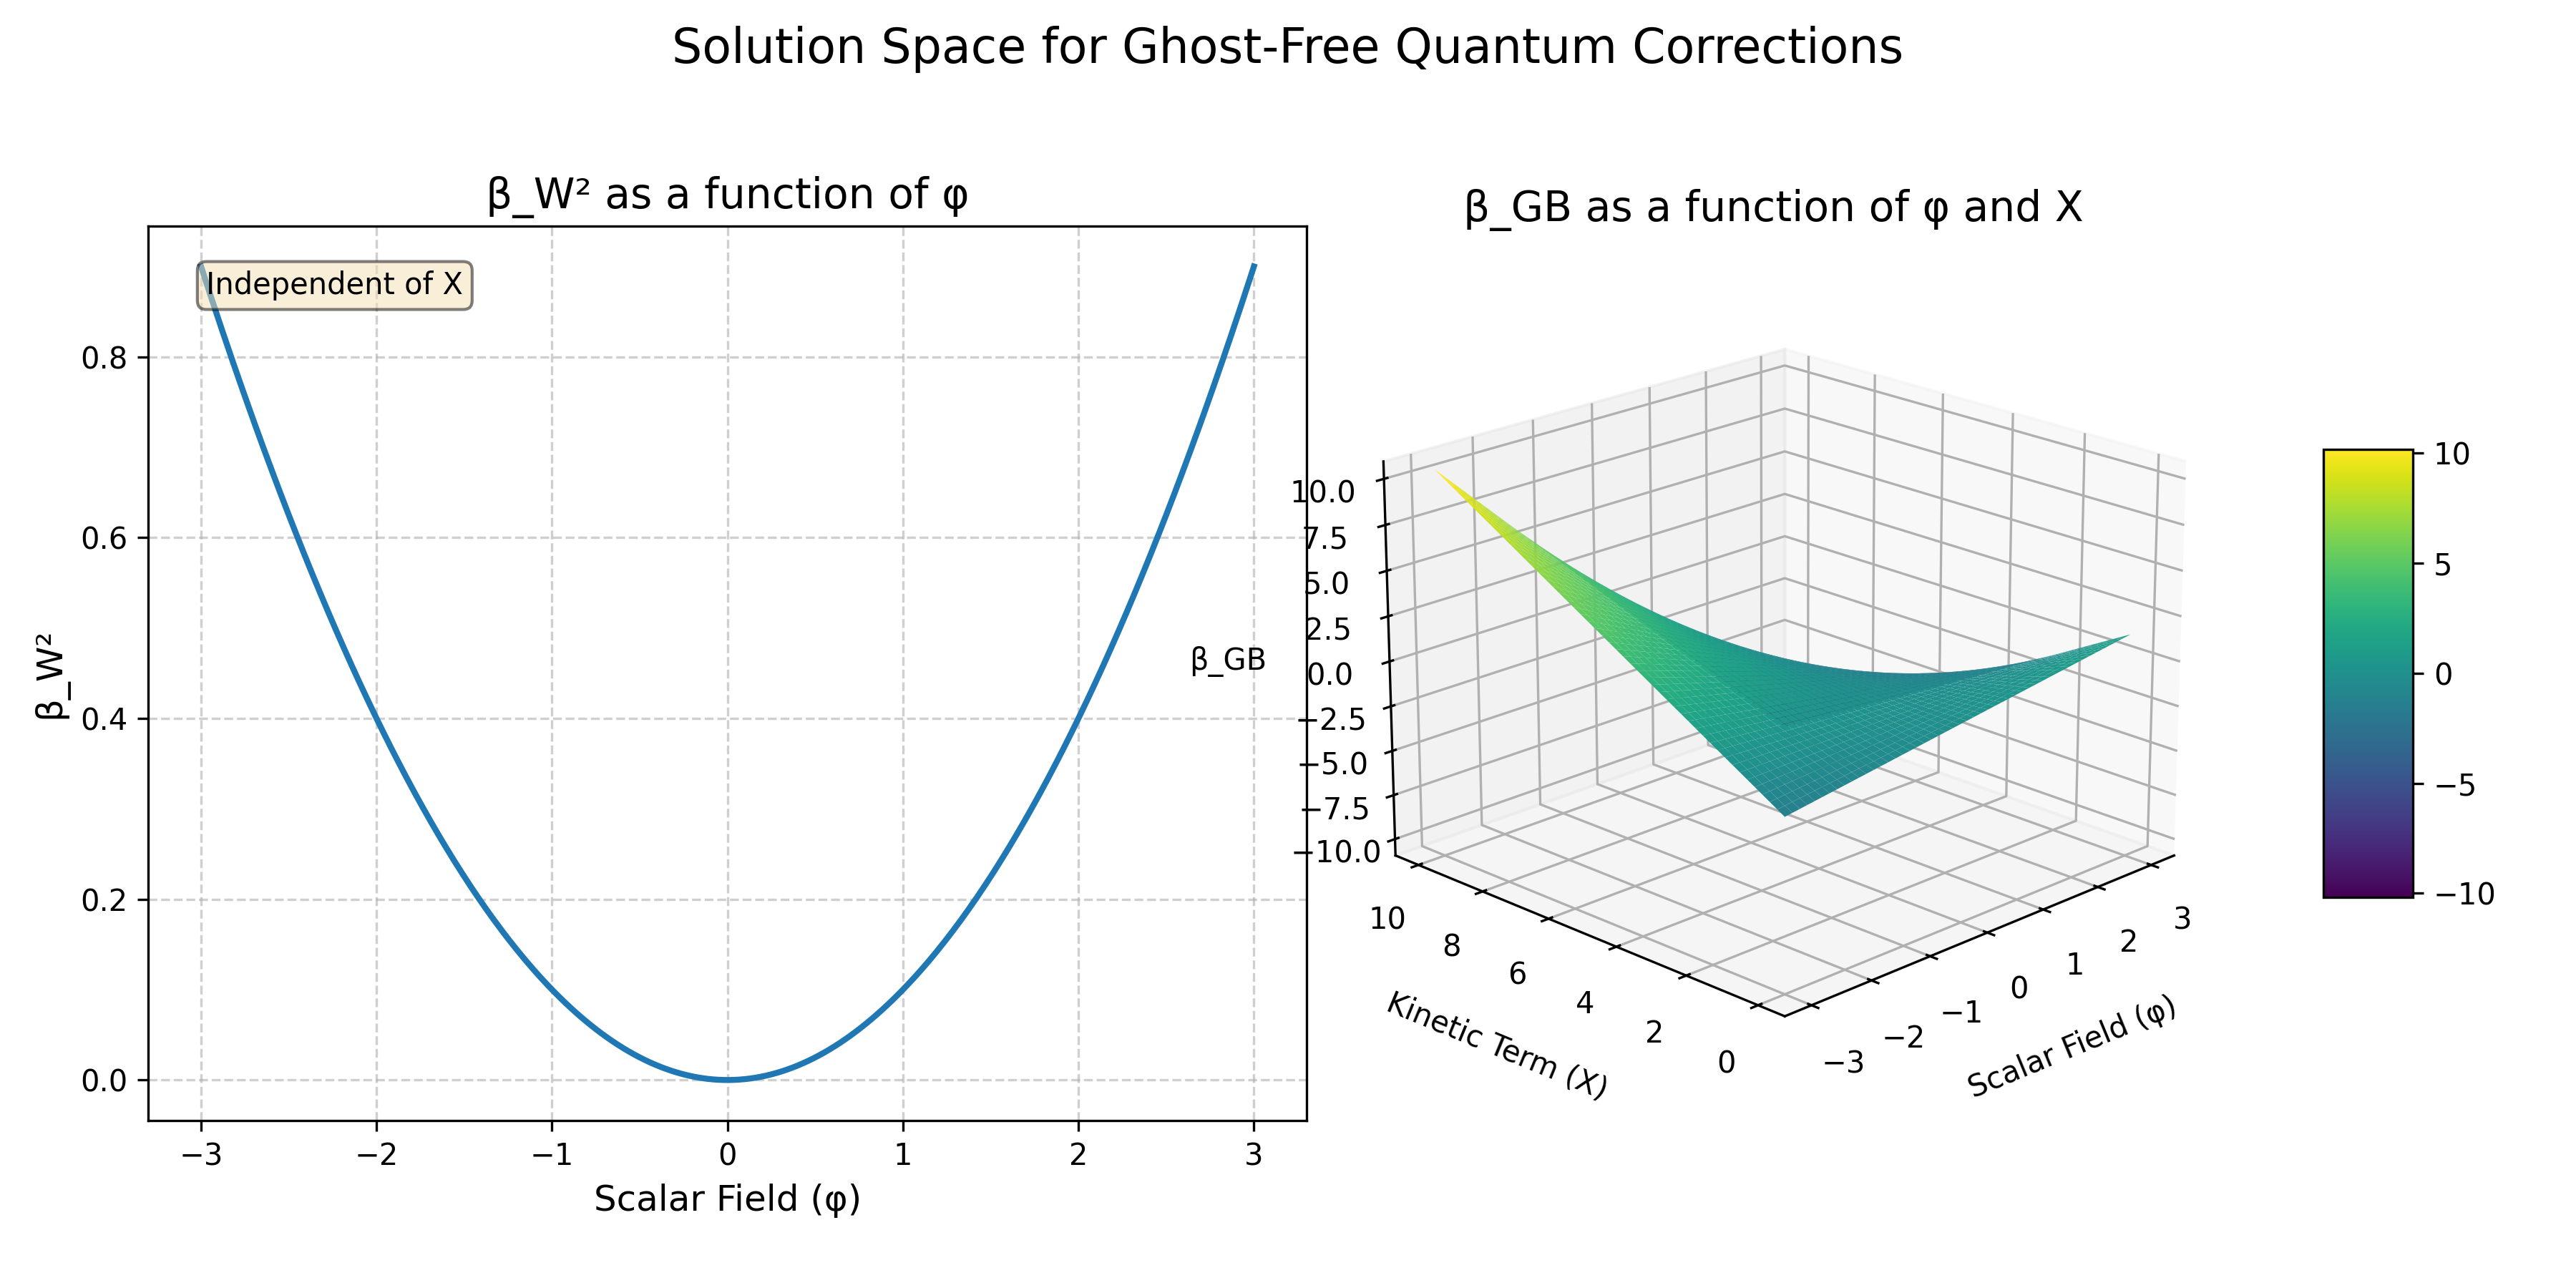
\includegraphics[width=0.5\textwidth]{../input_files/plots/solution_space_visualization_1_1772039099.png}
    \caption{The functional structure of quantum correction coefficients required for a ghost-free and gauge-invariant theory. The Weyl-squared coefficient, $\beta_{\text{W}^2}$, must be independent of the kinetic term $X$ (left), which in turn dictates that the Gauss-Bonnet coefficient, $\beta_{\text{GB}}$, must be linear in $X$ (right). This illustrates the specific, coupled functional dependence necessary to maintain the theory's physical viability.}
    \label{fig:functional_structure}
\end{figure}

In summary, our results demonstrate that the consistency of quantum-corrected scalar-tensor theories is guaranteed by extending the classical protective gauge symmetry to the full action. This principle of extended gauge invariance leads to a unique functional structure for the coefficients of the higher-derivative terms, thereby providing a clear and robust method for constructing physically viable gravitational effective field theories.

\section{Conclusions}
\label{sec:conclusions}
In this paper, we addressed the fundamental tension between the necessity of higher-derivative quantum corrections in scalar-tensor effective field theories and the stringent requirement of ghost-freedom. While classical DHOST theories are meticulously constructed to be free of the Ostrogradsky instability via a degeneracy condition, the inclusion of requisite curvature-squared operators, such as the Weyl-squared term, naively breaks the protective gauge symmetry responsible for this stability. We have resolved this tension by establishing a rigorous mathematical equivalence between the preservation of this gauge symmetry and the health of the theory's Hamiltonian structure.

Our method proceeded along two independent analytical paths. First, by demanding that the full action, including Gauss-Bonnet and Weyl-squared terms with general coefficients $\beta_{\text{GB}}(\phi, X)$ and $\beta_{W^2}(\phi, X)$, remain invariant under the protective gauge transformation of the classical theory, we derived a set of coupled partial differential equations for these coefficient functions. Second, we performed a first-principles Hamiltonian analysis using the ADM formalism. By imposing the primary and secondary constraints required to eliminate the Ostrogradsky ghost, we derived a separate set of conditions on the coefficients from the dynamical requirement of a well-posed theory.

The central result of our work is the proof that these two sets of conditions, one derived from an algebraic symmetry principle and the other from a dynamical stability analysis, are identical. Specifically, we found that both approaches demand that the Weyl-squared coefficient depend only on the scalar field, $\beta_{W^2}(\phi)$, and that the kinetic dependence of the Gauss-Bonnet coefficient be precisely linked to it via the relation $\partial_X \beta_{\text{GB}} = -2 \partial_\phi \beta_{W^2}$. This equivalence is a profound result, demonstrating that the gauge symmetry is not a fragile feature of the classical theory but is, in fact, the fundamental origin of Hamiltonian stability in the full quantum-corrected effective field theory.

From this work, we have learned that the consistency of gravitational EFTs is governed by a deep principle: the protective symmetries of the classical theory must be extended in a non-trivial way to encompass the higher-derivative quantum corrections. This finding elevates the symmetry principle from a model-building curiosity to a powerful and indispensable tool. It provides a clear and computationally tractable method for constructing ghost-free theories without resorting to a complete, and often prohibitively complex, Hamiltonian analysis. By demonstrating that gauge invariance and Hamiltonian stability are two manifestations of the same underlying physical principle, our work provides a robust guiding framework for navigating the vast landscape of modified gravity, ensuring that the theories we construct are not only phenomenologically interesting but also fundamentally consistent.

\bibliography{bibliography}{}
\bibliographystyle{aasjournal}

\end{document}
